% !TeX encoding = UTF-8
% !TeX program = pdflatex
% !BIB program = bibtex

%%% Um einen Artikel auf deutsch zu schreiben, genügt es die Klasse ohne
%%% Parameter zu laden.
\documentclass[english]{lni}
%%% To write an article in English, please use the option ``english'' in order
%%% to get the correct hyphenation patterns and terms.
%%% \documentclass[english]{class}
%%

\usepackage{booktabs}
\usepackage{pgfplots}

\pgfplotsset{width=12.5cm, height=5.3cm}

\begin{document}
%%% Mehrere Autoren werden durch \and voneinander getrennt.
%%% Die Fußnote enthält die Adresse sowie eine E-Mail-Adresse.
%%% Das optionale Argument (sofern angegeben) wird für die Kopfzeile verwendet.
\title[Which Rules Entail this Fact? An Efficient Approach Using RDBMSs]{Which Rules Entail this Fact? An Efficient Approach Using RDBMSs}
%%% \subtitle{From Facts to Rules using Relational Databases} % if needed
\author[Tim Gutberlet \and Janik Sauerbier]
{Tim Gutberlet\footnote{University of Mannheim, \email{tim.gutberlet@students.uni-mannheim.de}} \and
Janik Sauerbier\footnote{University of Mannheim, \email{janik.sauerbier@students.uni-mannheim.de}}}
\startpage{1} % Beginn der Seitenzählung für diesen Beitrag / Start page
\editor{B. König-Ries et al.} % Names of Editors
\booktitle{Datenbanksysteme für Business, Technologie und Web (BTW 2023)} % Name of book title
\yearofpublication{2023}
%%%\lnidoi{18.18420/provided-by-editor-02} % if known
\maketitle

\begin{abstract}
 In this paper, we focus on the problem of identifying all rules that entail a certain target fact given a knowledge graph and a set of previously learned rules. This problem is relevant in the context of link prediction and explainability. We propose an efficient approach using relational database technology including indexing, filtering and pre-computing methods. Our experiments demonstrate the efficiency of our approach and the effect of various optimizations on different datasets like YAGO3-10, WN18RR and FB15k-237 using rules learned by the bottom up rule learner AnyBURL. 
 
\end{abstract}
\begin{keywords}
Knowledge graphs \and Relational databases \and Link prediction \and Explainability.
\end{keywords}
%%% Beginn des Artikeltexts
\section{Introduction}
Knowledge graphs (KGs) are used in different fields from biomedical applications \cite{OpenBioLink} over applications in the context of social networks \cite{SocialNetworks} to semantic search applications \cite{SemanticSearch}. Learned rules over the KG describe patterns of the KG and allow for knowledge inference. This can be for example used to predict missing or additional information also known as the link prediction problem.

Identifying which previously learned rules of a KG entail certain target facts is an important problem for two main reasons. Firstly, to determine the confidence of an (unknown) fact, one must know from which rules it can be derived. The confidence of a fact refers to the probability that a particular fact within the graph is correct. Knowing the confidence is needed for rule-based link prediction models \cite{AnyBURL19}. Moreover, the confidence is used for building ensembles with embedding models \cite{RuleEmbeddingCombination1} and for improving embedding models \cite{RuleEmbeddingCombination2}. Secondly, it is generally helpful to be able to explain the connections between rules and (potential) facts. There is a significant need for a time-efficient approach to solve this problem. 


In this paper, we create and analyze an effective approach to this problem, using relational database technology. Our approach uses indexing, filtering and pre-computing methods tailored to the natural structure of a KG and its respective rules. To illustrate the performance of our approach, we ran several experiments on different KGs (YAGO3-10 \cite{YAGO3}, WN18RR \cite{WN18RR} and FB15k-237 \cite{FB15k-237}). Moreover, we show how different database setups impact the performance for different rule lengths. For the rule learning, we use AnyBURL, a fast bottom up rule learner for KGs \cite{AnyBURL19}.

\section{Preliminaries} 
A KG is a set of (subject, relation, object)-triples also called facts. There is a set of entities present as subjects and objects as well as a set of relations in a KG. Here is an example KG with the entities \(peter\), \(anna\) and \(germany\) and the relations \(livesIn\) and \(marriedTo\).

\begin{equation*} \label{eq:knowledgegraph}
\textbf{KG} = \{(anna,marriedTo, peter), (peter,bornIn,germany)\}\end{equation*}

For our purposes, we are concerned about first-order logic Horn rules, which describe patterns of KGs. Here are two example rules. We capitalize the variables and lowercase the constants representing entities.

\begin{equation} \label{eq:rule_1}
(X, citizenOf, germany) \leftarrow (X, bornIn, mannheim) 
\end{equation} 
\begin{equation} \label{eq:rule_2}
(X, livesIn, germany) \leftarrow (X, marriedTo, A_1), (A_1, bornIn, germany)
\end{equation}

Each rule has a head (e.g., \((X, citizenOf, germany)\)) consisting of one atom and a body (e.g., \((X, 
bornIn, mannheim)\)) consisting of one or more atoms. A grounding of a rule assigns values to all variables of the rule, resulting in a ground rule. A true body grounding refers to a grounding of the body of a rule for which all (ground) atoms appear in the KG. The problem we are solving is identifying all rules that entail certain target facts based on the KG and a previously learned set of rules. This means we are interested in whether there exists a true body grounding and the head atom can be unified with the target fact. To illustrate the problem, think of the following target fact.

\begin{equation*} \label{eq:target_1}
\textbf{Target fact} = (anna, livesIn, germany)
\end{equation*}


Rule (\ref{eq:rule_1}) does not entail this fact because its head atom cannot be unified with the target fact.
The head of rule (\ref{eq:rule_2}) can be unified with the target fact by assigning \(X = anna\). Therefore, it would entail the target fact if \(\exists A_1 ((anna, marriedTo, A_1) \wedge (A_1, bornIn, germany))\). The KG contains the facts \((anna, marriedTo, peter)\) and \((peter, bornIn, germany)\). Together with the target fact, this results in a true body grounding for rule (\ref{eq:rule_2}) with \(X = anna\) and \(A_1 = peter\). Therefore, rule (\ref{eq:rule_2}) is part of the solution.

\section{Proposed Approach}

The given KG is stored in one table of the relational database (\textit{kg\_table} with columns “sub” for subjects, “rel” for relations and “obj” for objects). The basic idea behind our approach is creating SQL queries which check whether a certain rule entails a certain target fact. Those individual queries are then combined using \textit{UNION ALL} operations over all rules, where the head can unify with the target fact. To improve this basic idea, we employ several optimizations listed below. This would be the query for rule (\ref{eq:rule_2}) and the target fact given in the preliminaries:

\textit{\textbf{SELECT} rule\_1 \textbf{FROM} kg\_table t0,  kg\_table t1 \textbf{WHERE} t0.sub = anna \textbf{AND} t0.rel = marriedTo \textbf{AND} t0.obj = t1.sub \textbf{AND} t1.rel = bornIn \textbf{AND} t1.obj = germany \textbf{LIMIT} 1;}

\subsection{Database Structure}
\label{database-structure}
Alternative to having one big table for all facts, our approach uses one table for each relation in the KG, with two columns for the subjects and the objects. This improves the performance by reducing the size of the B-trees of the indexes described in the following paragraph.

To speed up the search and enable direct access to the table contents through B-trees, we employ unique clustered indexes. We duplicate the knowledge graph tables and use once (subject, object) as key and once (object, subject) as key for the indexes. Within the generated SQL statements, the tables with the order (subject, object) are used in case of a fixed subject. The tables with the order (object, subject) are used in the case of a fixed object or no fixed subject and object. This ensures that the indexes are used efficiently.

\subsection{Advanced Rule Pre-filtering} 
Firstly, we only consider rules that can unify with the target fact for the query. This can be done by naively testing each rule. However, it can also be done more efficiently. The easiest way is storing each rule under its head as key in a hash map. The head stays unchanged, but we use “X” and “Y” as variable descriptors.

Let (s, r, o) be a target triple with the entities s and o and the relation r. Then we only use the rules stored under the keys \textit{(X, r, Y)}, \textit{(s, r, X)}, \textit{(X, r, o)} or \textit{(s, r, o)} for the query. Additionally, when it is true that s=o for the target, we also use the key \textit{(X, r, X)}. Instead of looping through n rules naively in O(n), this allows for initial filtering of the rules in O(1).

\subsection{Pre-computing of Expensive Rules}
\label{pre-computation}
As we will illustrate in our experiments, certain rules result in way more cost in terms of execution time than others. To address that, we pre-compute a portion of those rules. To identify the most expensive rules, we gather an independent set of n target facts from the KG and run their queries with the \textit{EXPLAIN ANALYZE} command to get the execution time for the individual rule sub-queries. Afterwards, we rank all rules which appear in the results by their average execution time multiplied with their number of appearances in the results. 

The top x\% of rules are then pre-computed, by calculating all potential assignments for variables in the rule head that form a grounding together with a set of facts from the KG. We then store these combinations in a table for the rule. If the subject or the object is a variable and the other one a constant, then the table only contains the column for the variable. For the implementation of the tables, we use materialized views to \(SELECT\) from the KG with all the conditions we already know from the rule. Consequently, the \(CREATE\) statement for pre-computing rule (\ref{eq:rule_2}) and the query for the target fact from the preliminaries would be: 

\textit{\textbf{CREATE MATERIALIZED VIEW} view\_rule\_1 \textbf{SELECT} t0.sub \textbf{AS} sub \textbf{FROM} kg\_table t0,  kg\_table t1 \textbf{WHERE} t0.rel = marriedTo \textbf{AND} t0.obj = t1.sub \textbf{AND} t1.rel = bornIn \textbf{AND} t1.obj = germany};


\textit{\textbf{SELECT} rule\_1 \textbf{FROM} view\_rule\_1  \textbf{WHERE} sub = anna \textbf{LIMIT} 1};

We exclude rules with one body atom, as pre-computing does not improve their performance. Moreover, we exclude rules with more than two body atoms, as those rules incur a pre-computing time two orders of magnitude higher than rules with two body atoms, while they only make up a fraction of the most expensive and frequent rules.

\section{Experiments}
The goal of our experiments is to benchmark the performance of our approach on different datasets and rulesets, as well as to measure the effects of different optimizations. Beyond that, we analyze the execution time for individual rules.

For the implementation of our approach, we used the open-source object-relational database system PostgreSQL. Additionally, we used Java with the PostgreSQL JDBC driver. The source code and datasets, we used for the experiments, can be found at https://github.com/timgutberlet/Which-Rules-Entail-This-Fact. We conducted all experiments on a Fujitsu Esprimo P957 (construction year 2017) with 32 GB RAM, 512 GB SSD, an Intel i7-7700 @ 3.6 GHz CPU and Ubuntu 22.04.1 LTS as an operating system. The rule learning with AnyBURL was mostly done with the standard configuration of AnyBURL-22 available at https://web.informatik.uni-mannheim.de/AnyBURL/. We only extended the limit of body atoms from one to three for acyclic rules to match the cyclic rules, as we do not intend to discriminate between them.

\subsection{Overall Performance}

\begin{table}[t]
\centering
\begin{tabular}{l|lll|lll}
\toprule
 & 10s & 50s  & 100s & \#entities & \#relations & \#facts of KG\\
\midrule
YAGO3-10 & 4 ms & 10 ms & 14 ms & 123,182 & 37 & 1,079,040\\
WN18RR & 35 ms & 65 ms & 77 ms & 40,943 & 11 & 86,835\\
FB15k-237 & 5 ms & 26 ms & 43 ms & 14,505 & 237 & 272,115\\
\bottomrule
\end{tabular}
\caption{Performance results (avg. execution time per target fact | dataset information)}
\label{tab:overall}
\end{table}

\begin{table}[t]
\centering
\begin{tabular}{l|lll|lll}
\toprule
 & 10s & 50s & 100s & 1 body atom & 2 body atoms & 3 body atoms\\
\midrule
YAGO3-10 & 27k & 107k & 165k & 82.8\% & 11.2\% & 6.0\%\\
WN18RR & 6k & 20k & 30k & 33.0\% & 23.9\% & 43.1\%\\
FB15k-237 & 33k & 135k & 252k & 53.9\% & 26.2\% & 19.9\%\\
\bottomrule
\end{tabular}
\caption{Composition of the rules (\# of rules | avg. share by \# of body atoms)}
\label{tab:rules}
\end{table}

As illustrated in \Cref{tab:overall}, our approach works for different datasets and rulesets learned by AnyBURL. For every dataset, we learned rules for 10s, 50s, and 100s (\Cref{tab:rules}). We use the training sets as the KGs and the test sets as the target triples (3k-20k triples). The validation sets (3k-20k triples) are used as target triples to create the rule rankings to pre-compute the top 1\% most expensive rules.

\subsection{Ablation Study - Optimizations} 

\begin{table}[t]
\centering
\begin{tabular}{lll}
\toprule
Experiment & Avg. execution time \\
\midrule
All optimizations enabled & 10 ms\\
\midrule
Advanced rule pre-filtering disabled & 55 ms\\
Tables for each relation disabled & 133 ms\\
Indexing disabled & 1720 ms\\
Pre-computing of expensive rules disabled & 16 ms\\

\bottomrule
\end{tabular}
\caption{Ablation study of optimizations using YAGO3-10 \& 107k rules}
\label{tab:ablation}
\end{table}


For the ablation study in \Cref{tab:ablation}, we use YAGO3-10 as the benchmark dataset and the AnyBURL 50s ruleset (107k rules). 

The “tables for each relation” optimization described in \ref{database-structure} specifically reduces the execution time for long rules. We tested this, by measuring the average execution time of different rule lengths in the version where the “table for each relation” optimization is enabled versus the version where the “table for each relation” optimization is disabled. In both runs, the rule pre-computing was disabled. In this experiment, the execution time for rules with one body atom is reduced by 12\%, for two body atoms by 25\% and for three body atoms by 74\% when the “table for each relation” optimization is enabled. This might be caused by the increased use of the indexes during execution for longer rules.

\subsection{Rule Quantile Performance Analysis} 

\begin{figure}[t]
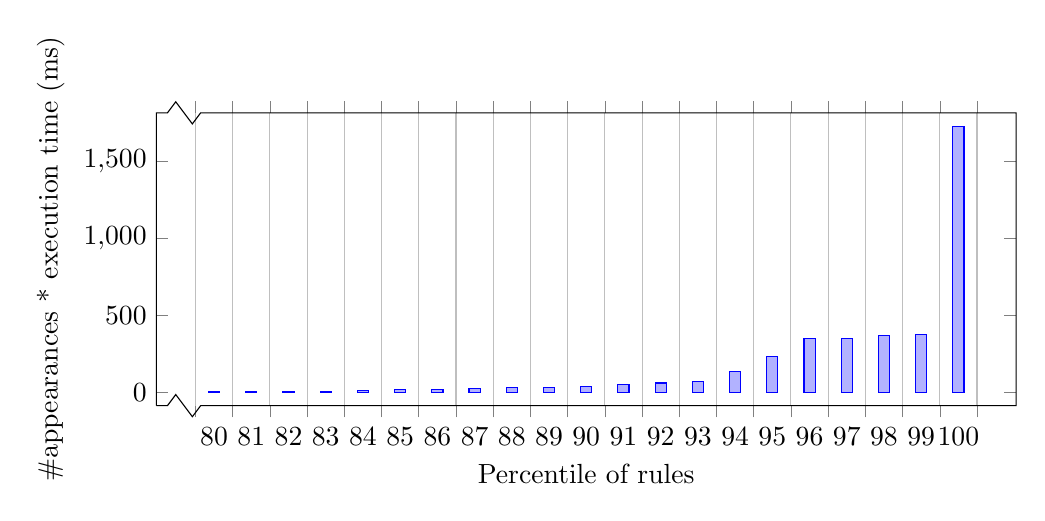
\begin{tikzpicture}
\begin{axis}[
	x tick label style={
		/pgf/number format/1000 sep=},
	ylabel=\#appearances * execution time (ms),
        xlabel=Percentile of rules,
	enlargelimits=0.05,
	legend style={at={(0.5,-0.1)},
	anchor=north,legend columns=-1},
	ybar interval=0.3,
        axis x discontinuity=crunch
]

\addplot 
	coordinates {(80, 3.909)
            (81, 4.361) (82, 4.934)
            (83, 6.515) (84, 10.682)
            (85, 16.204) (86, 17.215)
            (87, 23.746) (88, 28.900)
            (89, 32.942) (90, 38.231)
            (91, 49.141) (92, 60.599)
            (93, 71.221) (94, 135.862)
            (95, 235.4) (96, 348.644)
            (97, 352.313) (98, 367.095)
            (99, 374.032) (100, 1731.569)
            (101, 0)};
\end{axis}
\end{tikzpicture}
\caption{Quantile performance analysis of rules using YAGO3-10 \& 107k rules}
\label{fig:quantile-analysis}
\end{figure}


The quantile analysis in \Cref{fig:quantile-analysis} measures the total cost per rule after using the validation set as target triples, as described in \ref{pre-computation}. The total cost per rule is calculated by multiplying the number of appearances with the average execution time. Here, the number of appearances is a count for how often a rule appears as a result of the queries for all target triples.  It indicates that only few rules incur a major share of the cost. This ranking is used to determine the top x\% for the “pre-computing of expensive rules” optimization. In the given example (YAGO3-10 \& 107k rules), we achieved an 98.8\% execution time reduction for the pre-computed top 1\% rules. The pre-compution took five minutes. This reduced our average execution time from 16 ms to 10 ms, as illustrated in \Cref{tab:ablation}.


\section{Conclusions}

%
% the environments 'definition', 'lemma', 'proposition', 'corollary',
% 'remark', and 'example' are defined in the LLNCS documentclass as well.
%

We have designed an effective approach for finding all rules that entail a certain target fact given a knowledge graph and a set of previously learned rules. Our experiments specifically demonstrate the effect of indexing, filtering and pre-computing methods. Potential next steps include a further analysis of our approach on various datasets, a comparison of different database technologies (particularly triplestores), exploring the use of multithreading and creating a dedicated solution only using the main memory.

\textbf{Acknowledgement.} This paper would not have been possible without the exceptional support of our supervisor, Prof. Dr. Rainer Gemulla.

%%% Angabe der .bib-Datei (ohne Endung) / State .bib file (for BibTeX usage)
\bibliography{references} %\printbibliography if you use biblatex/Biber
\end{document}
